% This chapter should describe what was actually produced: the programs which were written, the hardware which was built or the theory which was developed. Any design strategies that looked ahead to the testing stage should be described in order to demonstrate a professional approach was taken.

% Descriptions of programs may include fragments of high-level code but large chunks of code are usually best left to appendices or omitted altogether. Analogous advice applies to circuit diagrams or detailed steps in a machine-checked proof.

% The implementation chapter should include a section labelled "Repository Overview". The repository overview should be around one page in length and should describe the high-level structure of the source code found in your source code repository. It should describe whether the code was written from scratch or if it built on an existing project or tutorial. Making effective use of powerful tools and pre-existing code is often laudable, and will count to your credit if properly reported. Nevertheless, as in the rest of the dissertation, it is essential to draw attention to the parts of the work which are not your own. 

% It should not be necessary to give a day-by-day account of the progress of the work but major milestones may sometimes be highlighted with advantage.

% practical contributions.
% present deadlocks \& performance tests.
% reusable modules.

% Live testing revealed many subtle bugs, deadlocks, and performance issues (memory usage, messages dropped due to bugs preventing leaders from always advancing) that were time consuming to debug. However they helped me to flesh out a pacemaker algorithm based on these ad-hoc fixes that we have proven both correctness and liveness for. I also improved the ease of implementability based on practicalities I discovered during implementation (eg. using node offset and hashes to compare nodes)

% --- directory forest stuff
\definecolor{foldercolor}{RGB}{124,166,198}

\tikzset{pics/folder/.style={code={%
	\node[inner sep=0pt, minimum size=#1](-foldericon){};
	\node[folder style, inner sep=0pt, minimum width=0.3*#1, minimum height=0.6*#1, above right, xshift=0.05*#1] at (-foldericon.west){};
	\node[folder style, inner sep=0pt, minimum size=#1] at (-foldericon.center){};}
	},
	pics/folder/.default={20pt},
	folder style/.style={draw=foldercolor!80!black,top color=foldercolor!40,bottom color=foldercolor}
}

\forestset{is file/.style={edge path'/.expanded={%
		([xshift=\forestregister{folder indent}]!u.parent anchor) |- (.child anchor)},
		inner sep=1pt},
	this folder size/.style={edge path'/.expanded={%
		([xshift=\forestregister{folder indent}]!u.parent anchor) |- (.child anchor) pic[solid]{folder=#1}}, inner ysep=0.6*#1},
	folder tree indent/.style={before computing xy={l=#1}},
	folder icons/.style={folder, this folder size=#1, folder tree indent=3*#1},
	folder icons/.default={12pt},
}
% ---
\textit{In this chapter we describe the architecture of our implementation (section \ref{architecture}), conclude our theoretical explanation of HotStuff by discussing the chained algorithm and the pacemaker (section \ref{moretheory}), present a full specification for HotStuff with a proof of correctness and liveness (section \ref{spec}), describe key optimisations implemented (section \ref{performance}), present our load generator and experiment scripts which will be used in evaluation (section \ref{benchcode}), and give an overview of the repository structure (section \ref{repo}).}

\section{System Architecture} \label{architecture}

\begin{figure}[h!]
\centering
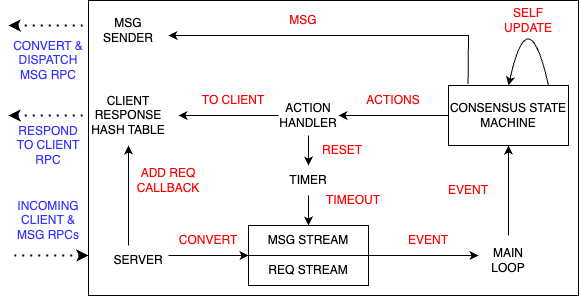
\includegraphics[scale=0.925]{nodediagram.png}
\caption{Architecture of a node.}
\label{nodediagram}
\end{figure}

In this section we present the system architecture that surrounds the core \textit{consensus} module, passing it new messages and client requests, and allowing it to send messages and respond to the client. This architecture is inspired by the OCons project\footnote{At the time I began implementation the OCons project was still under development, so I was unable to use the code in my project.} \cite{ocons}, which was developed by my project supervisor.

We will follow the path of an incoming request or message travelling through the system, as shown in figure \ref{nodediagram}.

\begin{description}
	\item \textit{Incoming message and client RPCs} --- the node responds to internal messages from other nodes, and requests from a client (or a load generator, as described in section \ref{loadgenerator}) containing new commands to be committed. The format of these RPCs is specified in a Cap'n Proto schema, in their custom markdown language.
	\item \textit{Server} --- each node operates as a server waiting for incoming RPCs. When the server receives an RPC it must be converted from Cap'n Proto types to internal types, and added to the \textit{message stream} or \textit{request stream}. If the RPC was a client request, a promise for a response is added to the \textit{client response hash table}; this will allow the system to respond to the client once the command is decided.
	\item \textit{Message and request streams\footnote{A stream is thread-safe implementation of a queue in Lwt.}} - messages and requests are added to separate streams so that messages can be prioritised. Internal messages represent a backlog of work that the system has not yet completed, so we follow the general design principle of clearing this backlog before accepting new work (client requests).
	\item \textit{Main loop} --- takes messages and requests from their respective streams, and delivers them to the \textit{consensus} module. This main loop ensures that the \textit{consensus} module is never run in parallel, which could lead to race conditions.
	\item \textit{Consensus module} --- takes incoming messages and requests, outputs \textit{actions} such as sending messages, and updates its own state. The module contains an implementation of the basic HotStuff algorithm (section \ref{hotstufftheory}), and the chained algorithm (chaining is discussed in section \ref{chaining}, and a full specification is given in section \ref{spec}); both share the same signature, so can be interchanged. The module uses the Tezos cryptography library (section \ref{tezos}) for signing messages, aggregating signatures, and checking quorum certificates.
	\item \textit{Action handler} --- takes the actions outputted by the \textit{consensus} module, and passes them to the appropriate handler. The three types of actions are: sending a message, responding to the client, and resetting the view timer.
	\item \textit{Message sender} --- asynchronously dispatches an RPC in a new thread. To do this it must convert internal types into Cap'n Proto types, and construct an RPC that matches the schema. The message sender maintains TCP connections with all other nodes, and in the event of the connection breaking repeatedly attempts to reconnect with binary exponential back-off times.
	\item \textit{Client request hashtable} --- allows client requests to be responded to. The hashtable maps each command's unique identifier to a promise, that will be awoken to respond to the original client request RPC once the command is committed.
	\item \textit{View timer} --- waits for a timeout to elapse then adds a view timeout message to the \textit{message stream}, so that it will be delivered to the \textit{consensus} module. The \textit{reset} action allows the timer to be reset for a new view.
\end{description}

\section{More HotStuff theory} \label{moretheory}
In this section we conclude our theoretical explanation of HotStuff by discussing chaining, and the pacemaker. As the pacemaker was not sufficiently specified in the original paper, we will draw on other sources to give a full explanation.

\subsection{Chaining} \label{chaining}

In this section we describe the \textit{chained} HotStuff algorithm, which is an optimised version of the basic algorithm described in section \ref{hotstufftheory} where different phases are pipelined. This is a standard optimisation for consensus algorithms that is described in the original paper \cite{yinHotStuffBFTConsensus2019}.

Pipelining phases both simplifies and optimises the basic algorithm. The phases in the basic algorithm were all very similar; they involved collecting votes from replicas to form a QC that then serves in later phases. Instead of having different phases as before, we can have a single \textit{generic} phase that collects votes, creates a \textit{generic QC}, and sends it to the next leader; now each view is the length of a single phase and a QC can serve in multiple phases concurrently. The only exception to this is the \textit{new-view} phase which is the same as in the basic algorithm.

\begin{figure}[h!]
\centering
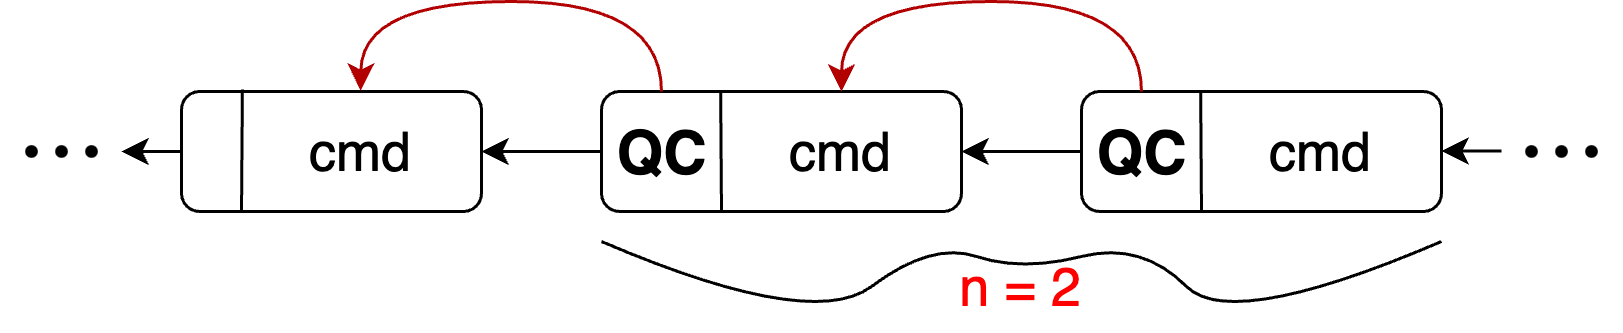
\includegraphics[]{nchain.png}
\caption{Sequence of nodes forming a 2-chain [label parent and justify links!!! fix font].}
\label{nchain}
\end{figure}

In each view a chain of nodes is extended, and different phases are carried out on nodes depending on how long a chain they form. For example, figure \ref{nchain}, shows a 2-chain, which means a proposal has already been through 2 phases\footnote{Not counting the new-view phase, as this can be considered to be the end of the previous view.}; this is the equivalent of being in the \textit{commit} phase in the basic algorithm.
% Figure \ref{nchain} shows a chain of nodes connected by `parent' links; every time we propose a value we extend the chain with a new node. Some node \textit{b} also contains a link to another node within \textit{b.justify.node}, which is the previous generic QC in the chain. In the event of a view-change a dummy node will be inserted in the chain which will cause a `gap' where some \textit{b.justify.node} pointer jumps over a dummy node. If some node \textit{b} has a QC that points to its direct parent with no `gap' in-between, then we say that it forms a \textit{one-chain}. In general, if we have $n$ such direct links without `gaps' we refer to this as an \textit{n-chain}, as shown above.

% To reproduce the behaviour of the unchained algorithm, on receiving a proposal for node \textit{b\textsuperscript{*}} a replica must look at \textit{b\textsuperscript{*}.justify.node} to see if it points to an \textit{n-chain}. It must take different actions depending on the length of the chain:
% [replace this with pseudocode describing implementation]
% \begin{itemize}
% \item zero-chain: this is equivalent to the \textit{prepare} phase from the unchained version, so the replica votes for the proposal only if it does not conflict with their \textit{lock}
% \item one-chain: this is equivalent to the \textit{pre-commit} phase from the unchained version, so the replica should store a \textit{key}
% \item two-chain: this is equivalent to the \textit{commit} phase, so the replica should \textit{lock} on the value proposed at the start of the two-chain
% \item three-chain: this is equivalent to the \textit{decide} phase, so the replica can execute the commands from the node at the start of the three-chain
% \end{itemize}

\subsection{Pacemaker} \label{pacemaker}

In this section we discuss the pacemaker, which is responsible for the liveness of the system; ensuring that it is able to makes progress. The original paper did not sufficiently specify the pacemaker mechanism, so we have synthesised information about pacemakers from different sources (including our own experimentation) to give a full specification of HotStuff in section \ref{spec}. Part of the pacemaker that we will explain in this section is the \textit{view-change} protocol, which allows the view of a faulty leader to be skipped; ours is based on the pacemaker for LibraBFT \cite{baudetStateMachineReplication2019}, which is explained in a talk by Ittai Abraham \cite{ittai}. We will also discuss how the pacemaker can be integrated with the HotStuff algorithm; we did this through our own modifications based on deadlocks encountered during implementation.

% The model of collecting a quorum of COMPLAIN messages to transition to the next view is based on the pacemaker for LibraBFT \cite{baudet_state_nodate}, and is described in section \ref{viewchange}. The rest of the pacemaker is designed to advance to the next view as soon as the system allows, and is based on ad-hoc fixes to deadlocks that were encountered during implementation.

The notion of a pacemaker and the properties it should posses were formalised in the Cogsworth byzantine view synchronisation protocol \cite{naorCogsworthByzantineView2021}; we will later prove that our pacemaker has these properties, and that they lead to liveness (section \ref{proof}). Pacemakers are related to the concept of a failure detector: a system that facilitates the detection of failed nodes \cite{chandraWeakestFailureDetector1996,chandraUnreliableFailureDetectors1996}. A pacemaker extends this idea, allowing it to be used in a multi-shot setting.

% We now present a reasonably formal proof that the modified pacemaker possesses qualities that ensure the liveness of the system. The first property (theorem \ref{viewsync}) ensures that there will always be opportunities for the system to make progress, and the second that the pacemaker cannot be controlled by a byzantine node (theorem \ref{syncvalid}). These properties are based on those described by Naor et. ~al~ in their paper presenting the Cogsworth byzantine view synchronisation protocol \cite{naor_cogsworth_2020}; their paper formalised the notion of a pacemaker and what qualities it should possess. [justify why we didn't implement cogsworth, it does not overlap with our ad-hoc fixes, these were original!!!]

\subsubsection{View-change protocol} \label{viewchange}

Once the view times out, nodes send a \textit{complain} message to the next leader and start a new timeout for the next view. Once the next leader achieves a quorum of \textit{complain} messages it collects them into a QC known as a \textit{view-change proof}. This leader can then send a \textit{view-change} message containing the \textit{view-change proof} to all replicas, who will respond by transitioning to the next view and sending a \textit{new-view} message to the new leader. The inclusion of the \textit{view-change proof} prevents liveness attacks by byzantine nodes that could otherwise attack the system by constantly causing view-changes to take place and preventing non-faulty leaders from making progress.

Crucially this protocol maintains the \textit{linear view change property} that HotStuff has $O(n)$ \textit{authenticator complexity}. Authenticator complexity measures the total number of threshold signatures and partial signatures in a view. This protocol requires $n - f$ partial signatures for the \textit{complain} messages, and a single threshold signature for the \textit{view-change} message, resulting in $O(n)$ authenticators overall.

\subsubsection{Integration}

Our approach to integrating the pacemaker is to advance a node to the next view as soon as possible once it has finished proposing or voting, or when it receives evidence that there are a quorum of nodes in a higher view. This means that the system does not require synchronised clocks; the nodes advance asynchronously as fast as the network allows.

During development we experimented with a prototype for a pacemaker that advanced views at a steady rate, but analysis of timing data indicated that this approach had inferior performance to our chosen design.

\section{Specification} \label{spec}

In this section we give a full specification of HotStuff based on the basic HotStuff algorithm (section \ref{hotstufftheory}), integrating chaining (section \ref{chaining}), and a pacemaker (section \ref{pacemaker}). We informally justify some of the changes made from the original algorithm, then give a proof of liveness for our modified algorithm.

This specification implements the consensus module as described in our discussion of the system architecture (section \ref{architecture}). This module receives messages and requests from the main loop, outputs actions (sending a message, responding to a client request, or resetting the view timer), and updates its own state.% We implement this as a \textit{match} statement over the different types of incoming messages and requests, returning a new state for the consensus machine, and a list of actions.

We present the pseudocode with our additions coloured in green and modifications in pink. We have only shown the main changes and not the other features and performance improvements we have made (such as batching), which are presented in section \ref{performance}.% The pseudocode is written to match the format of the original paper to allow for easier comparison, although as stated our actual implementation uses a match statement over the incoming messages and requests.

% \begin{algorithm}[h!]
% 	\caption{Modified HotStuff} \label{hotstuffalgorithm}
% 	\begin{algorithmic}[1]
% 	\Match{\textit{event}}
% 		\Case{\text{GENERIC} \textit{msg}}
% 			\color{Green}
% 			\If {$ msg.src = \text{GET{\large L}EADER}(\textit{msg.view}) \land \textit{msg.view} = curView$} \label{code_checkview}
% 				\color{black}
% 				\State $\textit{b\textsubscript{new}} \gets \textit{m.node}$
% 				\State $\textit{n} \gets \textit{b\textsubscript{new}.justify.node}$
% 				\If{$\textit{b\textsubscript{new}.height} > \textit{vheight} \land (\textit{b\textsubscript{new}}\ \text{extends}\ \textit{b\textsubscript{lock}} \lor \textit{n.height} > \textit{b\textsubscript{lock}.height})$}
% 					\State $\textit{vheight} \gets \textit{b\textsubscript{new}.height}$
% 					\State $ \text{SEND}(\text{GET{\large N}EXT{\large L}EADER}(), \text{VOTE{\large M}SG}\textsubscript{\textit{u}}(\text{GENERIC{\large A}CK}, \textit{b\textsubscript{new}}, \bot))$
% 				\EndIf
% 				\State $\textit{b''} \gets \textit{b\textsubscript{new}.justify.node}$
% 				\State $\textit{b'} \gets \textit{b''.justify.node}$
% 				\State $\textit{b} \gets \textit{b'.justify.node}$
% 				\State $\text{UPDATE{\large Q}C{\large H}IGH}(\textit{b\textsuperscript{*}.justify})$
% 				\If{$\textit{b'.height} > \textit{b\textsubscript{lock}.height}$}
% 					\State $\textit{b\textsubscript{lock}} \gets \textit{b'}$
% 				\EndIf
% 				\If{$(\textit{b''.parent} = \textit{b'}) \land (\textit{b'.parent} = \textit{b})$}
% 					\State $\text{ON{\large C}OMMIT}(\textit{b})$
% 					\State $\textit{b\textsubscript{exec}} \gets \textit{b}$
% 				\EndIf
% 				\color{Green}
% 				\If{$ \text{not}\ \text{IS{\large N}EXT{\large L}EADER}() $} \label{code_proposaltransition}
% 					\State $\text{ON{\large N}EXT{\large S}YNC{\large V}IEW}(\textit{curview} + 1)$
% 				\EndIf
% 			\EndIf
% 			\color{black}
% 		\EndCase
% 		\Case{\text{GENERIC{\large A}CK} \textit{msg}}
% 			\State $\textit{b.parent} \gets \text{branch extending with dummy nodes from}\ \textit{parent}\ \text{to height}\ \textit{curView}$
% 		\EndCase
% 		\Case{\text{NEW{\large V}IEW} \textit{msg}}
% 			\State $\textit{b.parent} \gets \text{branch extending with dummy nodes from}\ \textit{parent}\ \text{to height}\ \textit{curView}$
% 		\EndCase
% 		\Case{\text{CLIENT{\large R}EQ} \textit{req}}
% 			\State $\textit{b.parent} \gets \text{branch extending with dummy nodes from}\ \textit{parent}\ \text{to height}\ \textit{curView}$
% 		\EndCase
% 		\Case{\text{TIMEOUT} \textit{view}}
% 			\State $\textit{b.parent} \gets \text{branch extending with dummy nodes from}\ \textit{parent}\ \text{to height}\ \textit{curView}$
% 		\EndCase
% 		\Case{\text{COMPLAIN} \textit{msg}}
% 			\State $\textit{b.parent} \gets \text{branch extending with dummy nodes from}\ \textit{parent}\ \text{to height}\ \textit{curView}$
% 		\EndCase
% 		\Case{\text{\_} \textit{msg}}
% 			\State $\textit{b.parent} \gets \text{branch extending with dummy nodes from}\ \textit{parent}\ \text{to height}\ \textit{curView}$
% 		\EndCase
% 	\EndMatch
% 	\end{algorithmic}
% \end{algorithm}

\begin{algorithm}[h!]
	\caption{Modified HotStuff}\label{hotstuffalgorithm}
	\begin{algorithmic}[1]
	\Function{CREATE{\large L}EAF}{\textit{parent, cmd, qc}} \label{code_createleaf}
		\color{Magenta}
		\State $\textit{b.parent} \gets \text{branch extending with dummy nodes from}\ \textit{parent}\ \text{to height}\ \textit{curView}$
		\State $\textit{b.height} \gets \textit{curView} + 1$
		\color{black}
		\State $\textit{b.cmd} \gets \textit{cmd}$
		\State $\textit{b.justify} \gets \textit{qc}$
		\State \textbf{return} b
	\EndFunction
	\Procedure{UPDATE}{\textit{b\textsuperscript{*}}}
		\State $\textit{b''} \gets \textit{b\textsuperscript{*}.justify.node}$
		\State $\textit{b'} \gets \textit{b''.justify.node}$
		\State $\textit{b} \gets \textit{b\textsuperscript{*}.justify.node}$
		\State $\text{UPDATE{\large Q}C{\large H}IGH}(\textit{b\textsuperscript{*}.justify})$
		\If{$\textit{b'.height} > \textit{b\textsubscript{lock}.height}$}
			\State $\textit{b\textsubscript{lock}} \gets \textit{b'}$
		\EndIf
		\If{$(\textit{b''.parent} = \textit{b'}) \land (\textit{b'.parent} = \textit{b})$}
			\State $\text{ON{\large C}OMMIT}(\textit{b})$
			\State $\textit{b\textsubscript{exec}} \gets \textit{b}$
		\EndIf
	\EndProcedure
	\Procedure{ON{\large C}OMMIT}{\textit{b}}
		\If{$\textit{b\textsubscript{exec}.height} < \textit{b.height}$}
			\State $\text{ON{\large C}OMMIT}(\textit{b.parent})$
			\State $\text{EXECUTE}(\textit{b.cmd})$
		\EndIf
	\EndProcedure
	\Procedure{ON{\large R}ECEIVE{\large P}ROPOSAL}{$\text{MSG}\textsubscript{\textit{v}}(\text{GENERIC}, \textit{b\textsubscript{new}}, \textcolor{Magenta}{\textit{qc}})$} \label{code_onreceiveproposal}
		\color{Green}
		\If {$ v = \text{GET{\large L}EADER}(\textit{m.view}) \land \textit{m.view} = curView$} \label{code_checkview}
			\color{black}
			\State $\textit{n} \gets \textit{b\textsubscript{new}.justify.node}$
			\If{$\textit{b\textsubscript{new}.height} > \textit{vheight} \land (\textit{b\textsubscript{new}}\ \text{extends}\ \textit{b\textsubscript{lock}} \lor \textit{n.height} > \textit{b\textsubscript{lock}.height})$}
				\State $\textit{vheight} \gets \textit{b\textsubscript{new}.height}$
				\State $ \text{SEND}(\text{GET{\large L}EADER}(), \text{VOTE{\large M}SG}\textsubscript{\textit{u}}(\text{GENERIC}, \textit{b\textsubscript{new}}, \bot))$
			\EndIf
			\State $\text{UPDATE}(\textit{b\textsubscript{new}})$
			\color{Green}
			\If{$ \text{not}\ \text{IS{\large N}EXT{\large L}EADER}() $} \label{code_proposaltransition}
				\State $\text{ON{\large N}EXT{\large S}YNC{\large V}IEW}(\textit{curview} + 1)$
			\EndIf
		\EndIf
		\color{black}
	\EndProcedure
	\Procedure{ON{\large R}ECEIVE{\large V}OTE}{$\text{VOTE{\large M}SG}\textsubscript{\textit{v}}(\text{GENERIC{\large A}CK}, \textit{b}, \bot)$} \label{code_onreceivevote}
		\color{Green}
		\If {$ \text{IS{\large L}EADER}(\textit{m.view} + 1) \land \textit{m.view} \ge curView$} \label{code_checkleader}
			\color{black}
			\If {$\exists(v, \sigma') \in V\textcolor{Magenta}{\textsubscript{m.view}}[b]$}
				\State \textbf{return}
			\EndIf
			\State $V[b] \gets V\textcolor{Magenta}{\textsubscript{m.view}}[b] \cup \{(v, m.partialSig)\}$
			\If{$ |V\textcolor{Magenta}{\textsubscript{m.view}}[b]| \ge n - f$}
				\State $qc \gets QC(\{ \sigma | (v', \sigma) \in V\textcolor{Magenta}{\textsubscript{m.view}}[b]\})$
				\State $ \text{UPDATE{\large Q}C{\large H}IGH}(\textit{qc}) $
				\color{Green}
				\State $\text{ON{\large N}EXT{\large S}YNC{\large V}IEW}(\textit{m.view} + 1)$ \label{code_gotvotes}
				\color{black}
			\EndIf
		\EndIf
	\EndProcedure
	\Function{ON{\large P}ROPOSE}{$ \textit{b\textsubscript{leaf}}, \textit{cmd}, \textit{qc\textsubscript{high}}$} \label{code_onpropose}
		\State $b\textsubscript{new} \gets \text{CREATE{\large L}EAF}(\textit{b\textsubscript{leaf}, \textit{cmd}, \textit{qc\textsubscript{high}}, \textit{b\textsubscript{leaf}.height} + 1})$
		\State $ \text{BROADCAST}(\text{MSG}\textsubscript{\textit{v}}(\text{GENERIC}, \textit{b\textsubscript{new}}, \textcolor{Magenta}{\textit{qc\textsubscript{high}}})) $ \label{code_propose}
		\State \textbf{return} b\textsubscript{new}
	\EndFunction
	\end{algorithmic}
\end{algorithm}

\begin{algorithm}[h!]
	\caption{Modified Pacemaker}\label{pacemakeralgorithm}
	\begin{algorithmic}[1]
	\Function{GET{\large L}EADER}{} \label{code_getleader}
		\color{Green}
		\State $\textbf{return}\ \textit{curView}\ \text{mod}\ \textit{nodeCount}$
		\color{black}
	\EndFunction
	\Procedure{UPDATE{\large Q}C{\large H}IGH}{$\textit{qc'\textsubscript{high}}$}
		\If {$\textit{qc'\textsubscript{high}.node.height} > \textit{qc\textsubscript{high}} $}
			\State $ \textit{qc'\textsubscript{high}} \gets \textit{qc\textsubscript{high}} $
			\State $ \textit{b\textsubscript{leaf}} \gets \textit{qc'\textsubscript{high}.node}$
		\EndIf
	\EndProcedure
	\Procedure{ON{\large B}EAT}{$\textit{cmd}$}
		\If {$ \textit{u} = \text{GET{\large L}EADER}()$}
			\State $ \textit{b\textsubscript{leaf}} \gets \text{ON{\large P}ROPOSE}(\textit{b\textsubscript{leaf}}, \textit{cmd}, \textit{qc\textsubscript{high}})$
		\EndIf
	\EndProcedure
	\Procedure{ON{\large N}EXT{\large S}YNC{\large V}IEW}{$\textit{view}$} \label{code_onnextsyncview}
		\color{Green}
		\State $ \textit{curView} \gets \textit{view}$
		\State $ \text{RESET{\large T}IMER}(\textit{curView})$
		\State $ \text{ON{\large B}EAT}(\textit{cmds.take()})$ \label{code_takecmd}
		\color{black}
		\State $\text{SEND}(\text{GET{\large L}EADER}(), \text{MSG}\textsubscript{\textit{u}}(\text{NEW{\large V}IEW}, \bot, \textit{qc\textsubscript{high}}))$
	\EndProcedure
	\Procedure{ON{\large R}ECEIVE{\large N}EW{\large V}IEW}{$ \text{MSG}\textsubscript{\textit{u}}(\text{NEW{\large V}IEW}, \bot, \textit{qc'\textsubscript{high}}) $}
		\State $ \text{UPDATE{\large Q}C{\large H}IGH}(\textit{qc'\textsubscript{high}}) $
	\EndProcedure
	\color{Green}
	\Procedure{ON{\large R}ECIEVE{\large C}LIENT{\large R}EQUEST}{\text{REQ}(\textit{cmd})} \label{code_onreceiveclientreq}
		\State $ \textit{cmds.add(cmd)} $
	\EndProcedure
	\Procedure{ON{\large T}IMEOUT}{$ \textit{view} $} \label{code_ontimeout}
		\State $ \text{SEND}(\text{GET{\large N}EXT{\large L}EADER}(), \text{MSG}(\text{COMPLAIN}, \bot, \bot)) $ \label{code_timeout}
		\State $ \text{RESET{\large T}IMER}(\textit{view} + 1) $
	\EndProcedure
	\Procedure{ON{\large R}ECIEVE{\large C}OMPLAIN}{$ m = \text{MSG}(\text{COMPLAIN}, \bot, \bot) $} \label{code_onreceivecomplain}
		\If {$ \text{IS{\large L}EADER}(\textit{m.view} + 1) \land \textit{m.view} \ge \textit{curView}$}
			\If {$\exists(v, \sigma') \in C\textsubscript{m.view}[b]$}
				\State \textbf{return}
			\EndIf
			\State $C\textsubscript{m.view}[b] \gets C[b] \cup \{(v, m.partialSig)\}$
			\If{$ |C\textsubscript{m.view}[b]| = n - f$}
				\State $qc \gets QC(\{ \sigma | (v', \sigma) \in C\textsubscript{m.view}[b]\})$
				\State $\text{BROADCAST}(\text{MSG}(\text{NEXT{\large V}IEW}, \bot, \textit{qc}))$ \label{code_nextviewmsg}
			\EndIf
		\EndIf
	\EndProcedure
	\Procedure{ON{\large R}ECEIVE{\large A}NY}{$ m = \text{MSG}(*, *, \textit{qc}) $} \label{code_onreceiveany}
		\If {$ \textit{qc.view} \ge \textit{curView}$}
				\State $\text{ON{\large N}EXT{\large S}YNC{\large V}IEW}(\textit{qc.view} + 1)$ \label{code_gotqc}
		\EndIf
	\EndProcedure
	\end{algorithmic}
\end{algorithm}

\subsection{Changes}
We now informally justify some of the key changes made to the original algorithm, with a specific focus on the changes we made to integrate the pacemaker with HotStuff (section \ref{pacemaker}). Many of these changes were made to fix deadlocks encountered during implementation.

\begin{description}
	\item \textit{Algorithm \ref{hotstuffalgorithm}, line \ref{code_proposaltransition}} --- if a replica is the next leader, it waits to receive votes before transitioning to the next view. This prevents a deadlock where the leader transitions to the next view too early and ignores vote messages from an earlier view.
	\item \textit{Algorithm \ref{hotstuffalgorithm}, line \ref{code_checkleader}} --- a node collects vote messages from future views so that if it has fallen behind, it can receive a quorum of votes and catch up to the current view. This prevents an honest node falling behind and not being able to make progress in the view where it is the leader. Votes from different future views are stored in separate sets ($V\textcolor{Magenta}{\textsubscript{m.view}}$), to prevent votes from different views being used to form a QC.
	\item \textit{Algorithm \ref{hotstuffalgorithm}, line \ref{code_onpropose}} --- proposals now includes a QC, allowing replicas to catch up if they are in a lower view.
	\item \textit{Algorithm \ref{pacemakeralgorithm}, line \ref{code_getleader}} --- we have chosen to use a round-robin system to assign leaders to views.
	\item \textit{Algorithm \ref{pacemakeralgorithm}, line \ref{code_onnextsyncview}} --- as soon as a node transitions into a view where it is leader, ON{\large B}EAT is invoked, causing it to propose a new value.
	\item \textit{Algorithm \ref{pacemakeralgorithm}, line \ref{code_onreceiveany}} --- if a node receives any QC from a future view $v$, it can safely transition to view $v + 1$
\end{description}

\subsection{Proofs} \label{proof}

HotStuff works under a partially-synchronous system model (section \ref{hotstufftheory}), so the following proofs assume that global synchronisation time has been reached, and messages have a bounded latency of $\delta$.
[For this proof we consider the consensus machine (algorithm \ref{hotstuffalgorithm}) and the pacemaker (algorithm \ref{pacemakeralgorithm}), to be separate entities.] - relate this to cogsworth synchroniser!!!

[prove liveness with properties!!!]

\begin{theorem}[View synchronisation] \label{viewsync}
	There exists infinite views with honest leaders that all honest replicas will be in simultaneously, and have enough time to make progress.
\end{theorem}

\begin{proof}
	From lemma \ref{viewslemma} we have that we can always find future views $v_1$ and $v_2$ with honest leaders $l_1$ and $l_2$, and from lemma \ref{progressionlemma} we have that $l_1$ will eventually enter $v_1$. We argue that all honest replicas will simultaneously be in either $v_1$ or $v_2$. Consider the cases of how $l_1$ could have entered $v_1$:
	\begin{enumerate}
		\item $l_1$ received a quorum of votes (algorithm \ref{hotstuffalgorithm}, line \ref{code_gotvotes}) --- $l_1$ will broadcast a QC of votes that will be received by all honest replicas within $\delta$. These replicas will transition to $v_2$, and send a vote to $l_2$ which will also transition once it receives a quorum of votes. Hence all honest replicas will simultaneously be in $v_2$.
		\item $l_1$ receives QC of COMPLAINS from itself (algorithm \ref{hotstuffalgorithm}, line \ref{code_gotqc}) --- $l_1$ must have broadcast the NEXT{\large V}IEW message to all honest replicas; they will receive it within $\delta$ and all enter $v_1$ simultaneously.
	\end{enumerate}
	Once all honest replicas are in a view with an honest leader, they will only transition once they have made progress, or once they timeout, which shouldn't happen if the timeout is sufficiently long. Hence they will all be in the view long enough to make progress.
\end{proof}

\begin{figure}[h!]
	\centering
	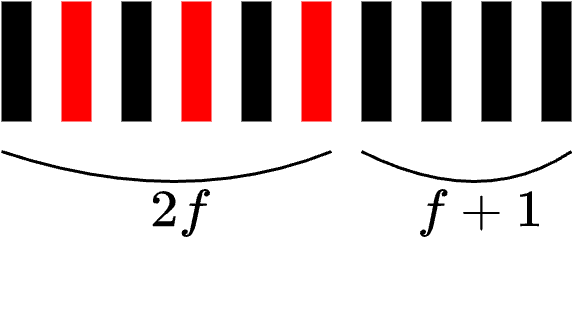
\includegraphics[]{lemma1.png}
	\caption{Example of round-robin leader allocation for $f = 1$. Red rectangles denote byzantine leaders. [maybe stripe red nodes so they appear in black and white???]}
	\label{lemma1diagram}
\end{figure}

\begin{lemma} \label{viewslemma}
	There exists an infinite number of consecutive assignments of two honest leaders to views. That is, we can always find future consecutive views $v_1$ and $v_2$ with honest leaders.
\end{lemma}

\begin{proof}
	We use a round-robin system to allocate leaders to views. If we attempt to alternate honest and byzantine leaders, there will always be $f + 1$ consecutive honest leaders left over (figure \ref{lemma1diagram}). Hence there will always be at least 2 consecutive honest leaders (the lemma holds trivially for $f = 0$).
\end{proof}

\begin{lemma} \label{progressionlemma}
	An honest replica $x$ will eventually enter a view where it is leader.
\end{lemma}

\begin{proof}
	In the event that a byzantine node is leader and tries to prevent honest nodes from transitioning to a higher view, the honest nodes will eventually timeout and send a COMPLAIN message to the next leader (algorithm \ref{pacemakeralgorithm}, line \ref{code_timeout}). This may repeat if the next leader is also byzantine. Eventually the COMPLAINs will be sent to an honest leader, that will send a NEXT{\large V}IEW message and transition all replicas into a new view (algorithm \ref{pacemakeralgorithm}, line \ref{code_nextviewmsg}). Since $x$ will always progress to a higher view, it will eventually reach a view where it is the leader [quickly justify that we cannot `skip ahead' without a qc from a future view].
\end{proof}

\begin{theorem}[Synchronisation validity] \label{syncvalid}
	The pacemaker will only advance the view if at least one honest consensus machine requests it to be advanced.
\end{theorem}

\begin{proof}
	This holds trivially for the calls to ON{\large N}EXT{\large S}YNC{\large V}IEW in algorithm \ref{hotstuffalgorithm}, as the view is advanced on the request of the consensus machine.

	The only other way the view can be advanced, is on the receipt of a QC (algorithm \ref{pacemakeralgorithm}, line \ref{code_gotqc}). For a QC to be formed a quorum of $n - f$ nodes must have complained or voted; at least one of these must have been an honest consensus machine that requested for the view to be advanced.
\end{proof}

% https://decentralizedthoughts.github.io/2021-09-30-distributed-consensus-made-simple-for-real-this-time/
\section{Practical challenges and optimisations} \label{performance}

In this section we give solutions to some of the practical challenges of implementing HotStuff, and describe optimisations we made to improve performance. The debugging and experimentation that led to these solutions was non-trivial; they involved extensive analysis of the program trace and timing data, and the development of different prototypes to compare performance.

One main practical consideration was designing the types and structure of the core consensus module (section \ref{architecture}), to implement the algorithm given in our specification (section \ref{spec}). Recall that this module takes as input messages and client requests (\textit{events}), and returns actions (such as sending a message) and an updated consensus state. We used \textit{variants} to tag the different types of events, with attached \textit{records} to store the body of the event (such as the node and QC of a proposal). The core algorithm is expressed as a \textit{match} statement to handle each type of event. The output from this is a list of actions (also implemented as variants), and a new state.

\subsection{Batching} \label{batching}
A standard technique to improve the goodput of a consensus algorithm is to \textit{batch} requests, making each node contain many commands instead of just one. This allows a single view to result in many commands being committed rather than just one.

In this section we discuss the practical challenges of implementing effective batching. A naive implementation of batching is simple to implement; instead of taking a single command from the queue to propose (algorithm \ref{pacemakeralgorithm}, line \ref{code_takecmd}), the whole queue can be batched into a single proposal. Analysis of the timing data for the naive implementation showed that it dramatically increased latency. The rest of this section describes further optimisations we made to make batching effective.

\subsubsection{Filtering} \label{filtering}
One optimisation that we implemented is \textit{filtering} incoming commands to prevent them being proposed by multiple nodes. This is achieved by nodes maintaining a set of commands that they have \textit{seen} in the proposals of other nodes, and filtering these commands from their proposal. The effectiveness of this optimisation demonstrated in our ablation study (section \ref{ablation}).

\begin{algorithm}[h!]
	\caption{Filtering implementation} \label{dedup}
	\begin{algorithmic}[1]
	\Procedure{ON{\large R}ECEIVE{\large P}ROPOSAL}{$\text{MSG}\textsubscript{\textit{v}}(\text{GENERIC}, \textit{b\textsubscript{new}}, \textit{qc})$}
		\If {$ v = \text{GET{\large L}EADER}(\textit{m.view}) \land \textit{m.view} = curView$}
			\State $ \textit{seen} \gets \textit{seen} \cup \textit{b\textsubscript{new}.cmds}$
			\State \textcolor{gray}{//\ \dots}
		\EndIf
	\EndProcedure
	\Procedure{ON{\large N}EXT{\large S}YNC{\large V}IEW}{$\textit{view}$}
		\State $ \textit{curView} \gets \textit{view}$
		\State $ \text{ON{\large B}EAT}(\textit{cmds} \setminus \textit{seen})$
		\State $ \textit{cmds} = \textit{seen} = \{\}$ \label{smalloptimisation}
		\State \textcolor{gray}{//\ \dots}
	\EndProcedure
	\Procedure{ON{\large R}ECIEVE{\large C}LIENT{\large R}EQUEST}{\text{REQ}(\textit{cmd})}
		\State $ \textit{cmds} \gets \textit{cmds} \cup \{\textit{cmd}\} $
	\EndProcedure
	\end{algorithmic}
\end{algorithm}

We give pseudocode for an implementation of filtering in algorithm \ref{dedup}. We use a set to store both the commands that are waiting to be proposed, and commands that have been seen, so that the difference can be efficiently computed. Also note the small optimisation on line \ref{smalloptimisation}: the \textit{seen} set can safely be emptied as the commands have already been filtered, reducing the amount of computation required to calculate the set difference next time.

This optimisation is effective as our load generator is send-to-all (section \ref{loadgenerator}), so a new command is added to the queue of all nodes, and may be included in the proposals of different nodes. Filtering out commands so that they are not proposed multiple times follows the general design principle:

\textbf{Design principle: } Attempt to minimise the amount of redundant work that the system carries out by screening incoming work to check that it actually needs to be done.

An alternative implementation of filtering that was prototyped was maintaining a set of commands that had been \textit{committed} rather than \textit{seen}, but this filtered out far fewer commands and did not significantly improve performance. This is likely because it takes several views for a command to be committed, and in this time multiple nodes may propose the same command and it will not be filtered.

\subsubsection{Batch sizes} \label{batchsizes}
We further improved the effectiveness of batching by limiting the size of each batch. We demonstrate that this approach improves performance in our study of the system with different batch size limits (section \ref{batchsizeseval}).

Implementing this feature requires minimal changes to algorithm \ref{dedup}, one simply has to take a subset of \textit{cmds} to propose instead of the whole set. It is important to take the oldest commands from \textit{cmds} to include in the proposal, so that older commands are not starved by newer ones, resulting in high latency. This can be accomplished by using an ordered set (such as a tree set), and ordering by command identifiers, which are ascending integers in our implementation.

The optimisation is effective because at higher message sizes the latency of Cap'n Proto serialisation increases (section \ref{capnpbenchmark}), so smaller batches can lead to better performance. There is an inherent trade-off between increasing batch size to commit more commands, and messages becoming slower due to increased serialisation latency.

\subsection{Nodes}
This section concerns the challenges of designing a suitable type for nodes\footnote{\textit{Node} is another word for log in this context.} that can be efficiently serialised by Cap'n Proto and sent over the network. Recall from our discussion of the system architecture (section \ref{architecture}) that the internal node type must be converted into a Cap'n Proto type in order to be serialised.

Nodes are implemented as OCaml records, and contain the fields \textit{parent}, \textit{cmds}, \textit{height}, and \textit{justify}. The \textit{justify} field contains a QC that contains another node inside it.

\subsubsection{Recursive types}
One difficulty encountered in converting internal types to Cap'n Proto types was that some nodes are recursive; the node stored inside the \textit{justify} field points to themselves. This is the case in the chained HotStuff algorithm (section \ref{chaining}); it has a recursive genesis node \textit{b\textsubscript{0}} that starts the chain of nodes. The genesis node \textit{b\textsubscript{0}} contains a hardcoded link to itself, so $ b_0.\textit{justify}.\textit{node} = b_0$.

This recursion poses a problem when carrying out the conversion between Cap'n Proto types and OCaml types. It is perfectly possible to define a recursive type in OCaml, so one can represent \textit{b\textsubscript{0}} inside the consensus state machine. However, the naive implementation of a function to convert this node into a Cap'n Proto type will not terminate, as it will infinitely recurse into the field $ b_0.\textit{justify}.\textit{node} $.

A simple solution to this problem is to add a flag to the Cap'n Proto schema \textit{is\_b\textsubscript{0}}; when this flag is enabled then the node is assumed to be equal to \textit{b\textsubscript{0}}. This prevents \textit{b\textsubscript{0}} from ever having to be converted into a Cap'n Proto type or being sent over the network, it can instead be reconstructed as a recursive type in the consensus state machine of the receiver.

\subsubsection{Node offsets}
In order to reduce memory usage, we replaced the \textit{node} record inside the \textit{node.justify.node} field with an integer offset into the chain. This dramatically decreased the memory usage of the function to convert from internal types to Cap'n Proto types. The inefficiency of this function was revealed through profiling the memory usage of the program using Memtrace  (section \ref{testing}).

The source of this problem was the inefficient design of the \textit{node.justify} field, which contained a whole node inside it. As shown in figure \ref{nchain}, each node has two links to previous nodes in the chain through the \textit{parent} field and the \textit{node.justify.node} field. By having each of these fields contain a whole \textit{node} record, much of the chain had multiple redundant copies, resulting in a very bloated \textit{node} object that was very expensive to convert.

A solution to this problem is to store an integer offset to a node inside the \textit{justify} field rather than a \textit{node} record. This offset represents how many \textit{parent} links away the node is, and so can be used to reconstruct all of the original information. To implement this another type \textit{node\_justify} was added, that is identical to \textit{qc}, but with the field \textit{node} replaced with \textit{node\_offset}. One must then convert between the \textit{node\_justify} and \textit{qc} types to reconstruct the original data and follow the \textit{node.justify.node} link.

\subsubsection{Node equality} \label{equality}
One optimisation implemented was storing a \textit{digest} field in the node that is a hash over all of the other fields\footnote{Notably the hash can be computed over the \textit{digest} field of the parent node rather than recursing through the whole chain.}, enabling efficient equality checking of nodes. This means that two nodes can be compared by their digests without having to recurse through the entire chain; the digests being equal cryptographically guarantees that the whole chains are equal. The need for this optimisation was discovered through profiling the memory usage of the node equality function using Memtrace.

\subsubsection{Node truncation} \label{truncation}
We implemented node truncation in order to reduce the size of nodes being sent over the network, cutting off older parts of the chain that the receiver already knows about. This is effective because the size of messages being sent is a bottleneck for our implementation (section \ref{capnpbenchmark}). The effectiveness of this optimisation demonstrated in our ablation study (section \ref{ablation}).

In order to truncate the node, our implementation recurses into the node's \textit{parent} field, then deletes the field at some chosen depth. The entire node can then be reconstructed at the receiver, by `splicing' it back together with \textit{b\textsubscript{exec}}, which contains the node up to the point that has been executed. Splicing together the nodes is done by recursing into the truncated node until it is equal to \textit{b\textsubscript{exec}}, then setting the deleted parent field to \textit{b\textsubscript{exec}}. The node equality function will still work on truncated nodes because of our optimisation to use digests (section \ref{equality}); a node will still have the same digest once it is truncated.

One practical challenge of this approach is choosing a suitable depth such that there is enough information at the receiver to reconstruct the whole chain. If there is a gap between the truncated node and \textit{b\textsubscript{exec}} at the receiver, this will lead to commands being missed out and not executed. This is a problem in the event that some node becomes isolated from the rest; it must be able to catch up to the others once the network partition is healed.

To overcome this problem we use a TCP-style approach. We include a field containing the height of the \textit{b\textsubscript{exec}} node to the \textit{propose}, \textit{new-view}, and \textit{complain} messages. Each node maintains a list of the \textit{b\textsubscript{exec}} height of every other node. When making a proposal, the leader takes the minimum height from this list, and truncates the node up to that depth. This ensures that every node that receives the proposal has enough information to reconstruct the entire log.

There are some cases when the leader does not receive the latest \textit{b\textsubscript{exec}} of every other node before it makes a proposal. This means that the leader will not truncate the node as much as it could have. We optimised this by having a node send the entire list of all stored \textit{b\textsubscript{exec}} heights rather than just its own, allowing the heights to propagate around the system more quickly.

% \subsection{Connections}
% talk about capabilities?
% when to set up connections? use promises
% https://outlook.office.com/mail/id/AAQkADc5ODY2YTdlLTQ3NGMtNDVmOS05ZDAxLWNhYzkwMjU2MThhZAAQAEXEcHtcUNFFo%2FRcUtQcSmc%3D

\section{Implementing for evaluation} \label{benchcode}
% Benchmarking code
% discuss open loop vs closed loop clients
% avoid coordinated ommision by using open loop clients
% section 3: https://dl.acm.org/doi/pdf/10.1145/3447851.3458739

\textit{In this section we describe the infrastructure that will be used to evaluate our system in chapter \ref{evaluation}, including the scripting developed to automate running experiments.}

\subsection{Load generator} \label{loadgenerator}

\begin{figure}[h]
\centering
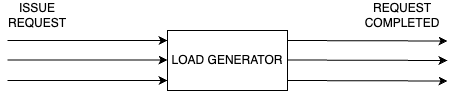
\includegraphics[]{openloop.png}
\caption{Open-loop load generator.}
\label{openloop}
\end{figure}

\begin{figure}[h]
\centering
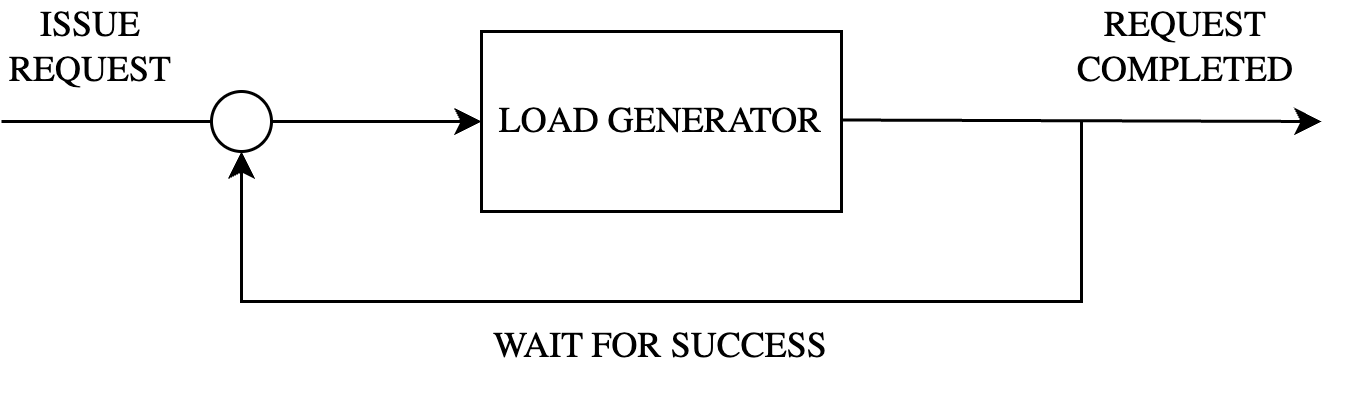
\includegraphics[]{closedloop.png}
\caption{Closed-loop load generator.}
\label{closedloop}
\end{figure}

The load generator is responsible for sending client requests to the nodes of the system. One is able to vary the throughput that the load generator drives the system at, and the duration that it runs for before it sends a \textit{kill} messages to the nodes, ending the test. It is also responsible for timing and calculating statistics.

\begin{description}
	\item \textit{Throughput} --- the number of requests sent by the load generator each second.
	\item \textit{Goodput} --- the number of requests that are responded to each second. This is calculated by number of responses divided by the time difference between the first response and the end of the test.
	\item \textit{Latency} --- the amount of time it takes between sending a request and receiving a response. The load generator reports both mean and standard deviation of latencies.
\end{description}

The load generator is open-loop (figure \ref{openloop}), which means that it dispatches a request every $\delta$ seconds for the duration of the experiment, where $\delta = \frac{1}{\textit{throughput}}$. This is in contrast to a closed-loop generator (figure \ref{closedloop}), which must wait until it receives a response in order to send the next request. An open-loop load generator is more useful for our experiments as it allows us to overload the system and test its limits, whereas a closed-loop load generator waits for responses from the system, so cannot overload it.

Our load generator is \textit{send-to-all}, meaning that a command is sent to all nodes. An alternative is \textit{send-to-one}, where a command is sent to a single node which is chosen at random. Send-to-all reduces latency as the next leader will have been sent the command, and may chose to propose it. In send-to-one it may take several views until the node that the request was sent to becomes the leader.

The load generator uses Lwt to asynchronously dispatch requests, and stores a promise that will be fulfilled with their response. In the case of send-to-all the promises waiting on a response from each node are combined using \textit{Lwt.pick}, meaning that the first node to respond will fulfil the promise and the rest will be ignored. Before beginning the experiment the load-generator sends `dummy' requests to each node until all of them have sent a response; this ensures that all nodes are properly up and running before we start the experiment, reducing start-up effects.

\subsection{Experiment scripts} \label{experimentscripts}
Python scripts are used to automate the running of experiments. These scripts start the nodes and the load generator, wait for the experiment to run, kill the processes, run a script to plot graphs, then start the next experiment.

Different experiments may vary input variables such as throughput, batch size, and number of nodes. The script takes every permutation. Each experiment is repeated several times to reduce variance. Experiments are run in a random order so that if there is interference for some part of the test, this is not correlated with the parameters of the experiment, making anomalies easier to spot.

\subsection{Logging framework}
We developed a logging framework that stores the time taken for important parts of the program to execute, and outputs key statistics such as the mean and standard deviation at the end of the test. This was essential for analysing the performance of the system to develop the optimisations described in section \ref{performance}.

The logging framework helped to reduce the effect of \textit{probing effects}, where the behaviour of a system is altered by the act of measuring it. Our previous approach printed the time taken throughout the execution of the program; since printing takes signficant CPU time this resulted in probing effects. Notably, the print statements were not in-between the statements that measured the time taken, but they caused delays to happen in other parts of the program (presumably when the buffers were being flushed).

\textbf{Design principle: } Minimise probing effects by carrying out the minimum possible amount of work in critical areas of the program, storing data, and moving work (such as outputting statistics) to less critical areas of the program.

\section{Repository Overview} \label{repo}

\begin{small}
\begin{forest}
	for tree={font=\sffamily, grow'=0,
	folder indent=0.9em, folder icons,
	edge=densely dotted}
	[src
		[\ consensus,
			[consensus\_chained\_impl.ml, is file]
			[consensus\_impl.ml, is file]
			[consensus.ml, is file]
			[consensus.mli, is file]
			[crypto\_util.ml, is file]
			[types.ml, is file]
			[types.mli, is file]
			[util.ml, is file]
		]
		[\ experiments
			[\ data]
			[\ graphs]
			[plot.py, is file]
			[runExperiments.py, is file]
		]
		[action\_handler.ml, is file]
		[api\_wrapper.ml, is file]
		[api\_wrapper.mli, is file]
		[hs\_api.capnp, is file]
		[load\_gen.ml, is file]
		[main.ml, is file]
		[net.ml, is file]
		[README.md, is file]
		[server.ml, is file]
		[types.ml, is file]
		[util.ml, is file]
	]
\end{forest}
\end{small}

The \textit{src} directory contains files implementing the main components described in the system architecture (section \ref{architecture}). This includes the server (\textit{server.ml}), main loop (\textit{main.ml}), action handler \textit{action\_handler.ml}, and the message / request sender (\textit{net.ml}). It also contains the schema for RPCs (\textit{hs\_api.capnp}) and code to convert between internal types and Cap'n Proto types (\textit{api\_wrapper.ml}).

Inside the \textit{consensus} folder is a module with implementations of the basic and chained HotStuff algorithms, sharing a common signature (\textit{consensus.mli}). There is also a utility code that allows the use of the \textit{consensus} module types with cryptography functions (\textit{crypto\_util.ml}).

The \textit{experiments} folder is where the data from running experiments is outputted to, and it contains scripts for running experiments and plotting graphs.

In order to run an experiment, first follow the instructions in \textit{README.md} to set up your environment. You can then run experiments by executing \textit{python3 runExperiments.py}, and modify this script to vary the input parameters such as throughput and experiment time. These scripts will run on Linux and MacOS, but will have to be modified to work on Windows.